\chapter[The 8$^{\text{th}}$ of March 2024]{}
\minitoc
\section{Mixed formulation}
\subsection{To do}
\begin{itemize}
    \item Recompute the experiments with $\alpha=0.0$. We don't need to Jacobian-based regularisation at the moment and since everything is super sensitive, it might make a difference in the results.
    \item Use normalised version of the $l_2$ error.
    \begin{itemize}
        \item In the parametric version, the computation of the normalised $\mathcal{L}_2$ error is already implemented
    \end{itemize}
\end{itemize}

\subsection{To think about}
\begin{itemize}
    \item How could we share the mesh for $u$ and $du$? We want the mesh coordinates to be effected by both loss terms. Also, some of the nodes are not shared by both variables. How to deal with this in our code?
    \item Is mixed-formulation solution equal to exact solution at the mesh nodes?
\end{itemize}

\section{2D domain }
\subsection{To do}
\begin{itemize}
    \item Triangular mesh. 
    \item Implement the reference element. For each training point $x$, find cell ID $i$. For cell $i$, get the coordinates of nodes and compute $L_i$ coordinates. Based on them, get the position of $x$ in reference element - $\xi$. Evaluate the shape functions, defined on the reference element, for $\xi$. Do the interpolation. \emph{I need to study the details. }
    
\end{itemize}

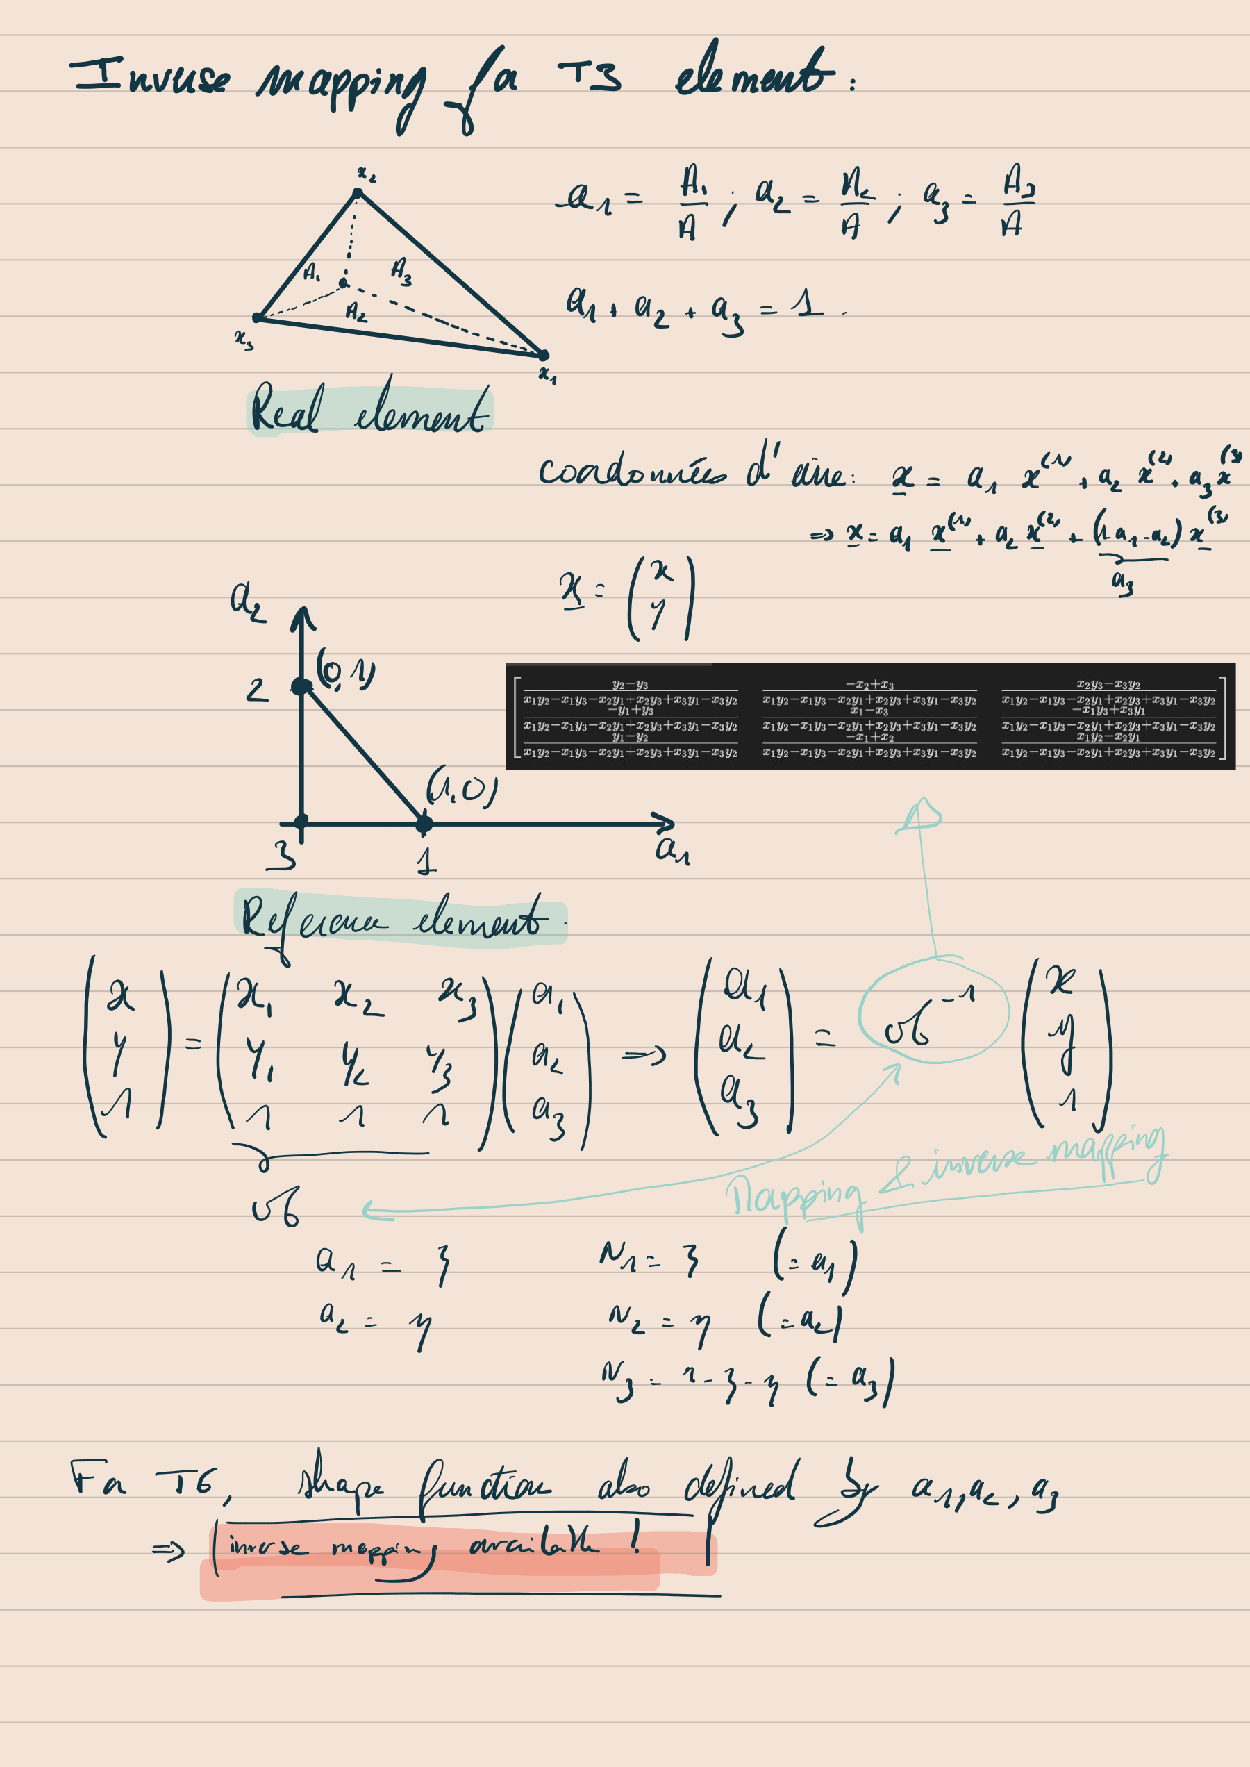
\includepdf[pages={1}]{Figures/InverseMappingT3.pdf}

\section{TODO Parametric}

\begin{itemize}
    \item Multi scale Tensor decomposition (Since modes can live on different meshes)
    \item Non-linear interpolation
    \item Non-linear potential to minimise
    \item Using mixed formulation
\end{itemize}
\section{``Big picture''}

If we can make this tool robust, it can dissociate the interpolation aspect from the solving of the PDE and give access to a high level tool in the sens that coding a solver would not be required but only writing the expression of the loss would be needed.

\begin{itemize}
    \item In the same sens that no one codes a linear solver but uses linear algebra libraries this be used as a replacement for non linear solvers with mesh adaptivity and parametric representation built into it
    \item Allow to use tensor decomposition and other technique without having to explicitly write the linearised problem and the iterative non-linear solver
    \item TODO: investigates its behaviour regarding snap-back and snap-through problems
\end{itemize}
